\chapter{Tools and Libraries}
\paragraph{} \textbf{OpenCV} is an open-source library for computer vision. It is used for capturing image, and extract features from it which ultimately leads to feature extraction and object detection.
\paragraph{} \emph{Grayscale and thresholding} of image is also done using OpenCV. Also capping by colour, Canny edge detection, erosion and dilation, contour search, and moments (to find centre of frame) are implemented using CV.


\begin{figure}[H]
  \centering
    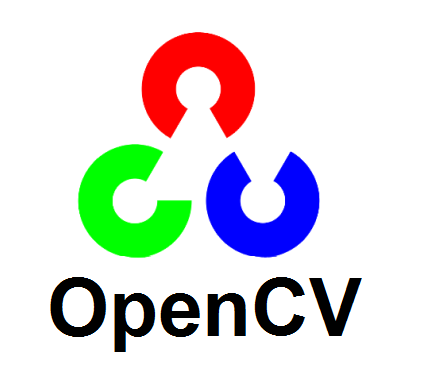
\includegraphics[scale=0.4]{project/images/cv}
  \caption{\textbf{OpenCV}}
\end{figure}

\paragraph{} Python language is used along with numpy distribution for numerical computation. Also Scipy is used for final distance/depth calculation.

\begin{figure}[H]
	\centering
	
\includegraphics[scale=0.4]{project/images/py}
	\caption{\textbf{Numpy \& Python}}
\end{figure}


